%note: don't split this document up with include{...}

\section{GUI-Entwürfe}

\begin{figure}[H]
\caption{GUI vor Ausführung der Analyse (Muss-Kriterien)}
\centering
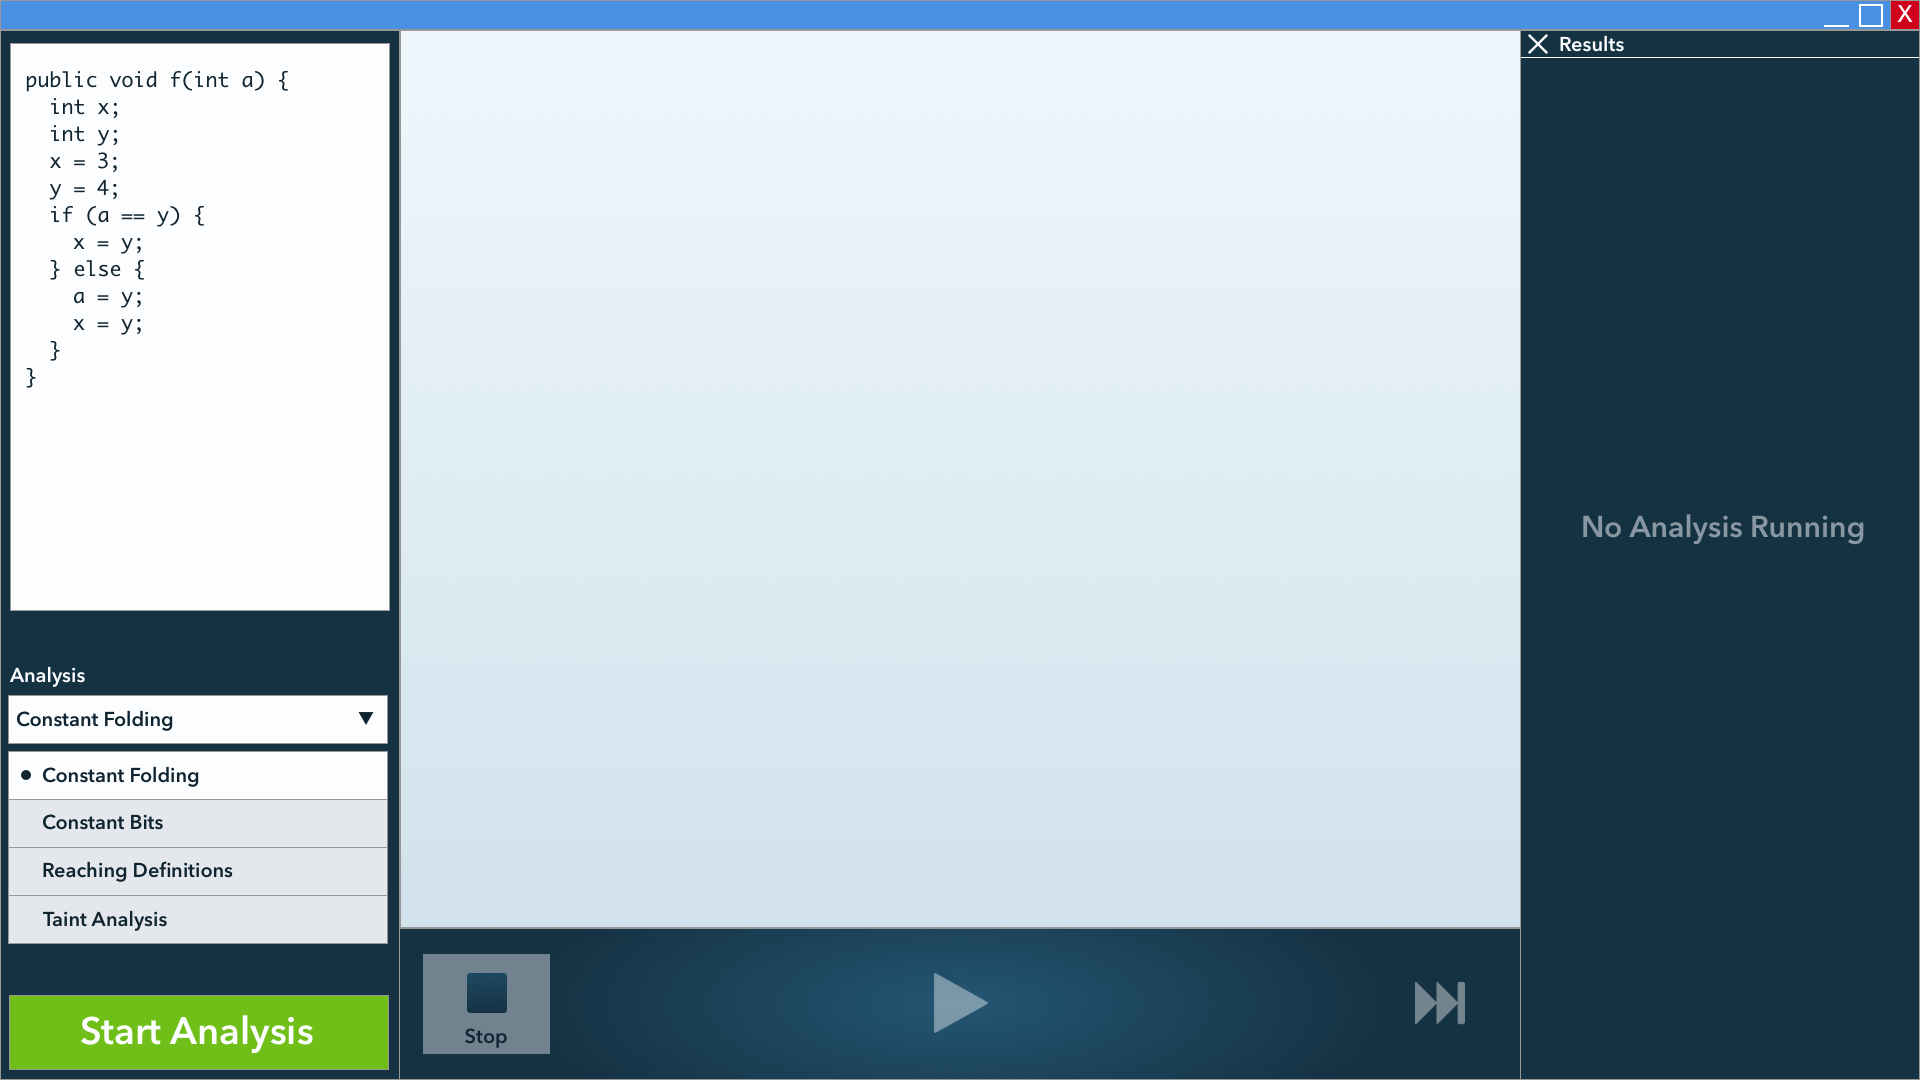
\includegraphics[angle=90, width=0.8\textwidth]{empty-muss}
\end{figure}

\begin{figure}[H]
\caption{GUI vor Ausführung der Analyse (Kann-Kriterien)}
\centering
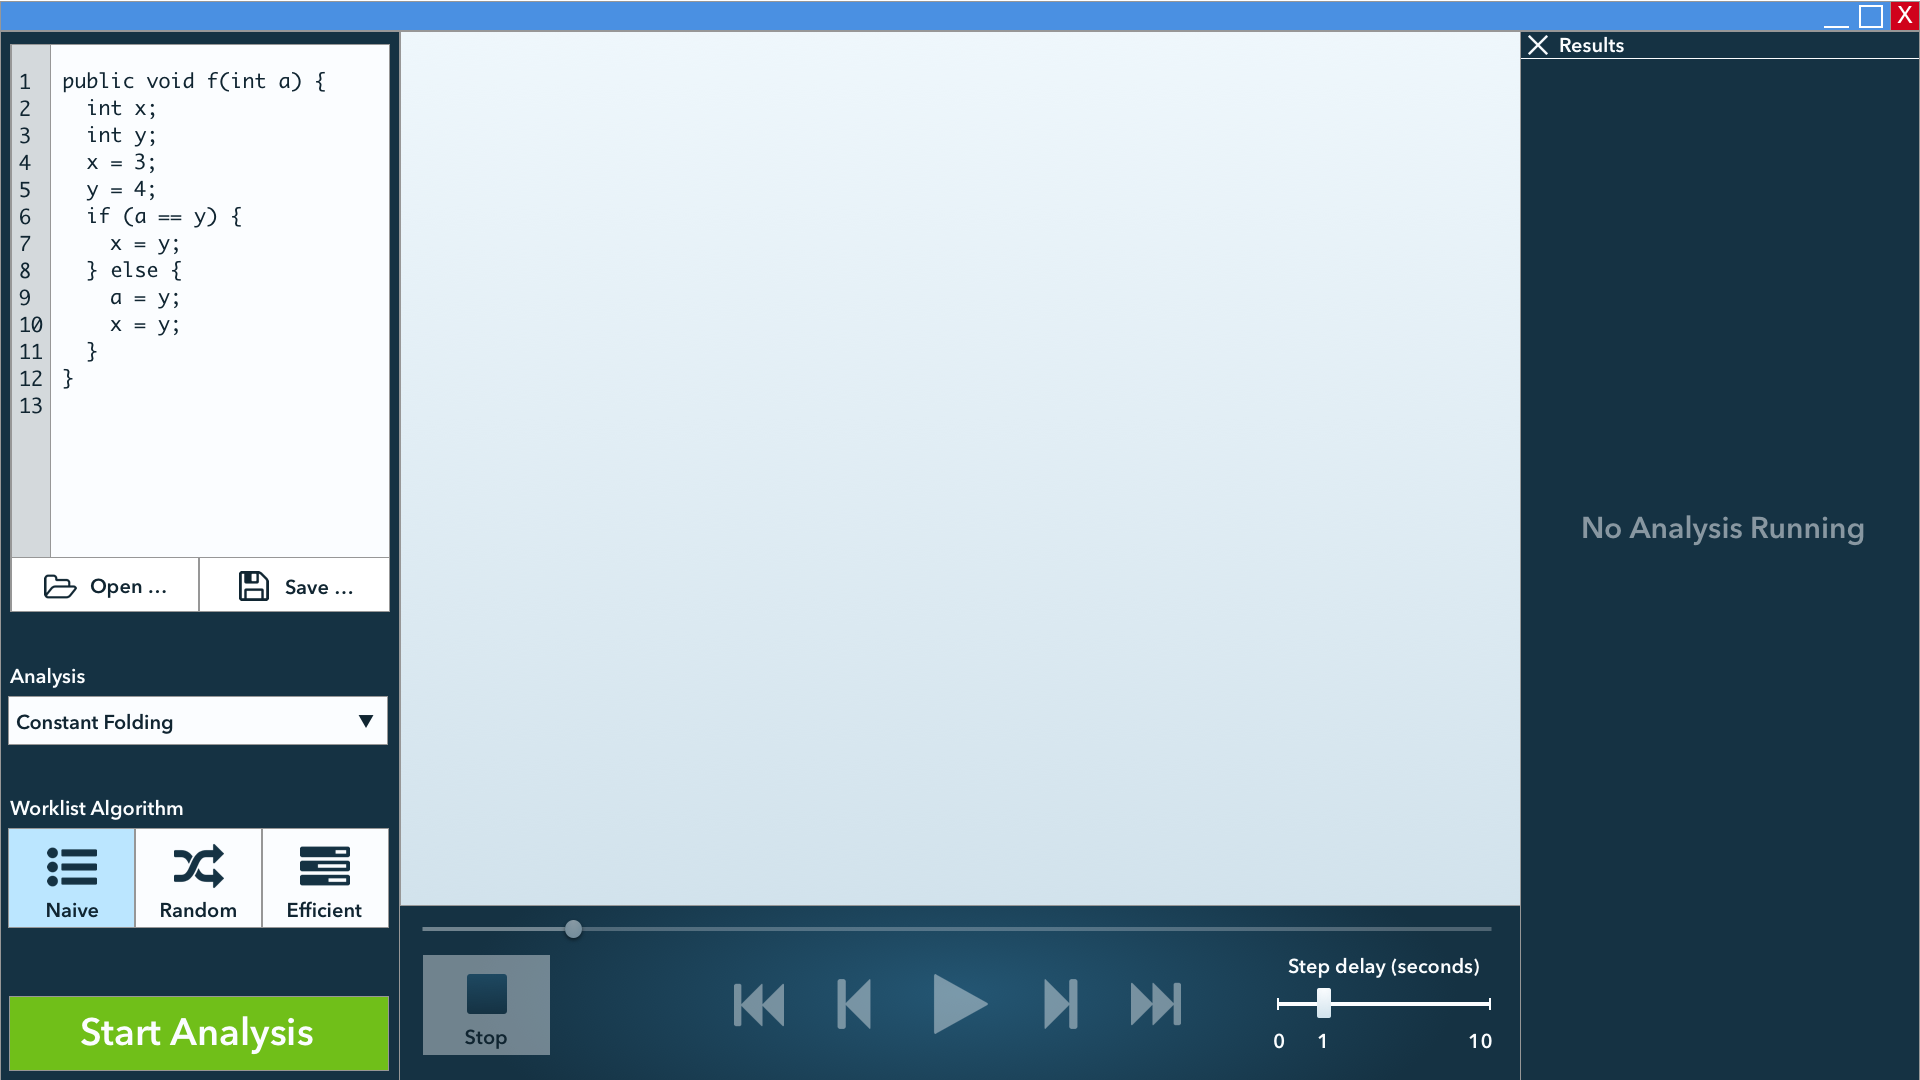
\includegraphics[angle=90, width=0.8\textwidth]{empty-kann}
\end{figure}

\begin{figure}[H]
\caption{GUI während Ausführung der Analyse (Muss-Kriterien)}
\centering
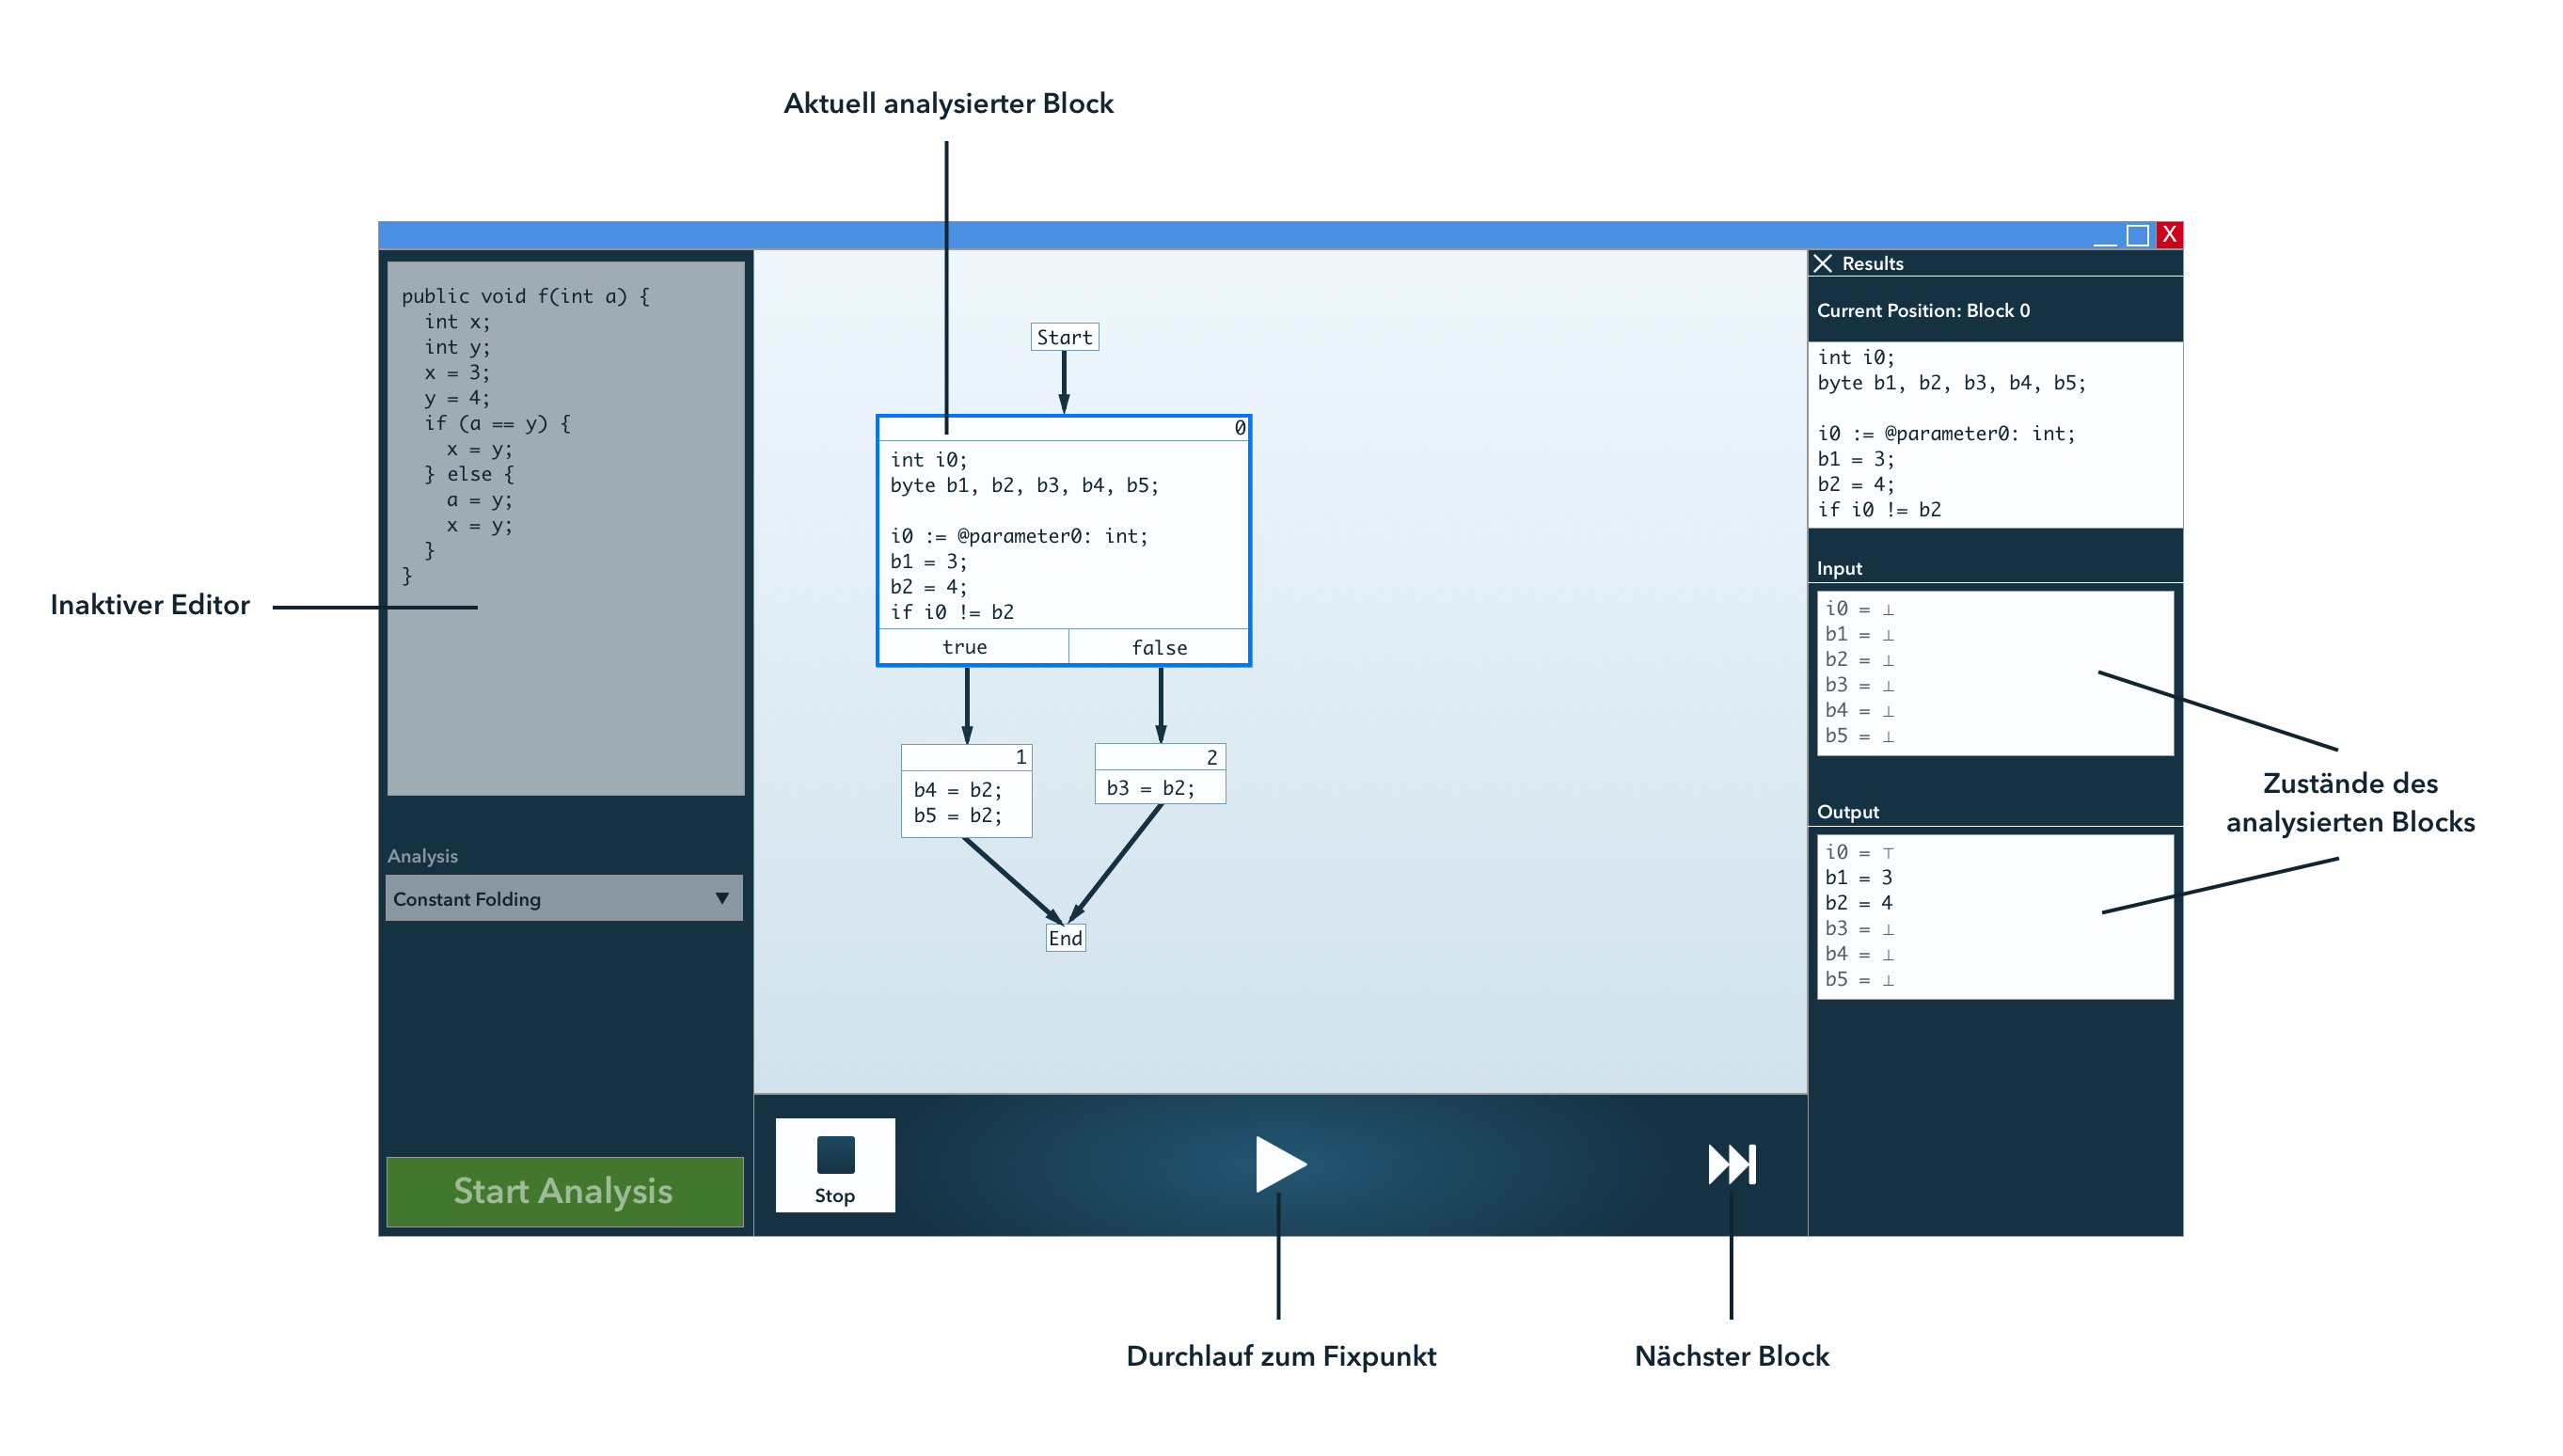
\includegraphics[angle=90, width=0.93\textwidth]{annotated-muss}
\end{figure}

\begin{figure}[H]
\caption{GUI während Ausführung der Analyse (Kann-Kriterien)}
\centering
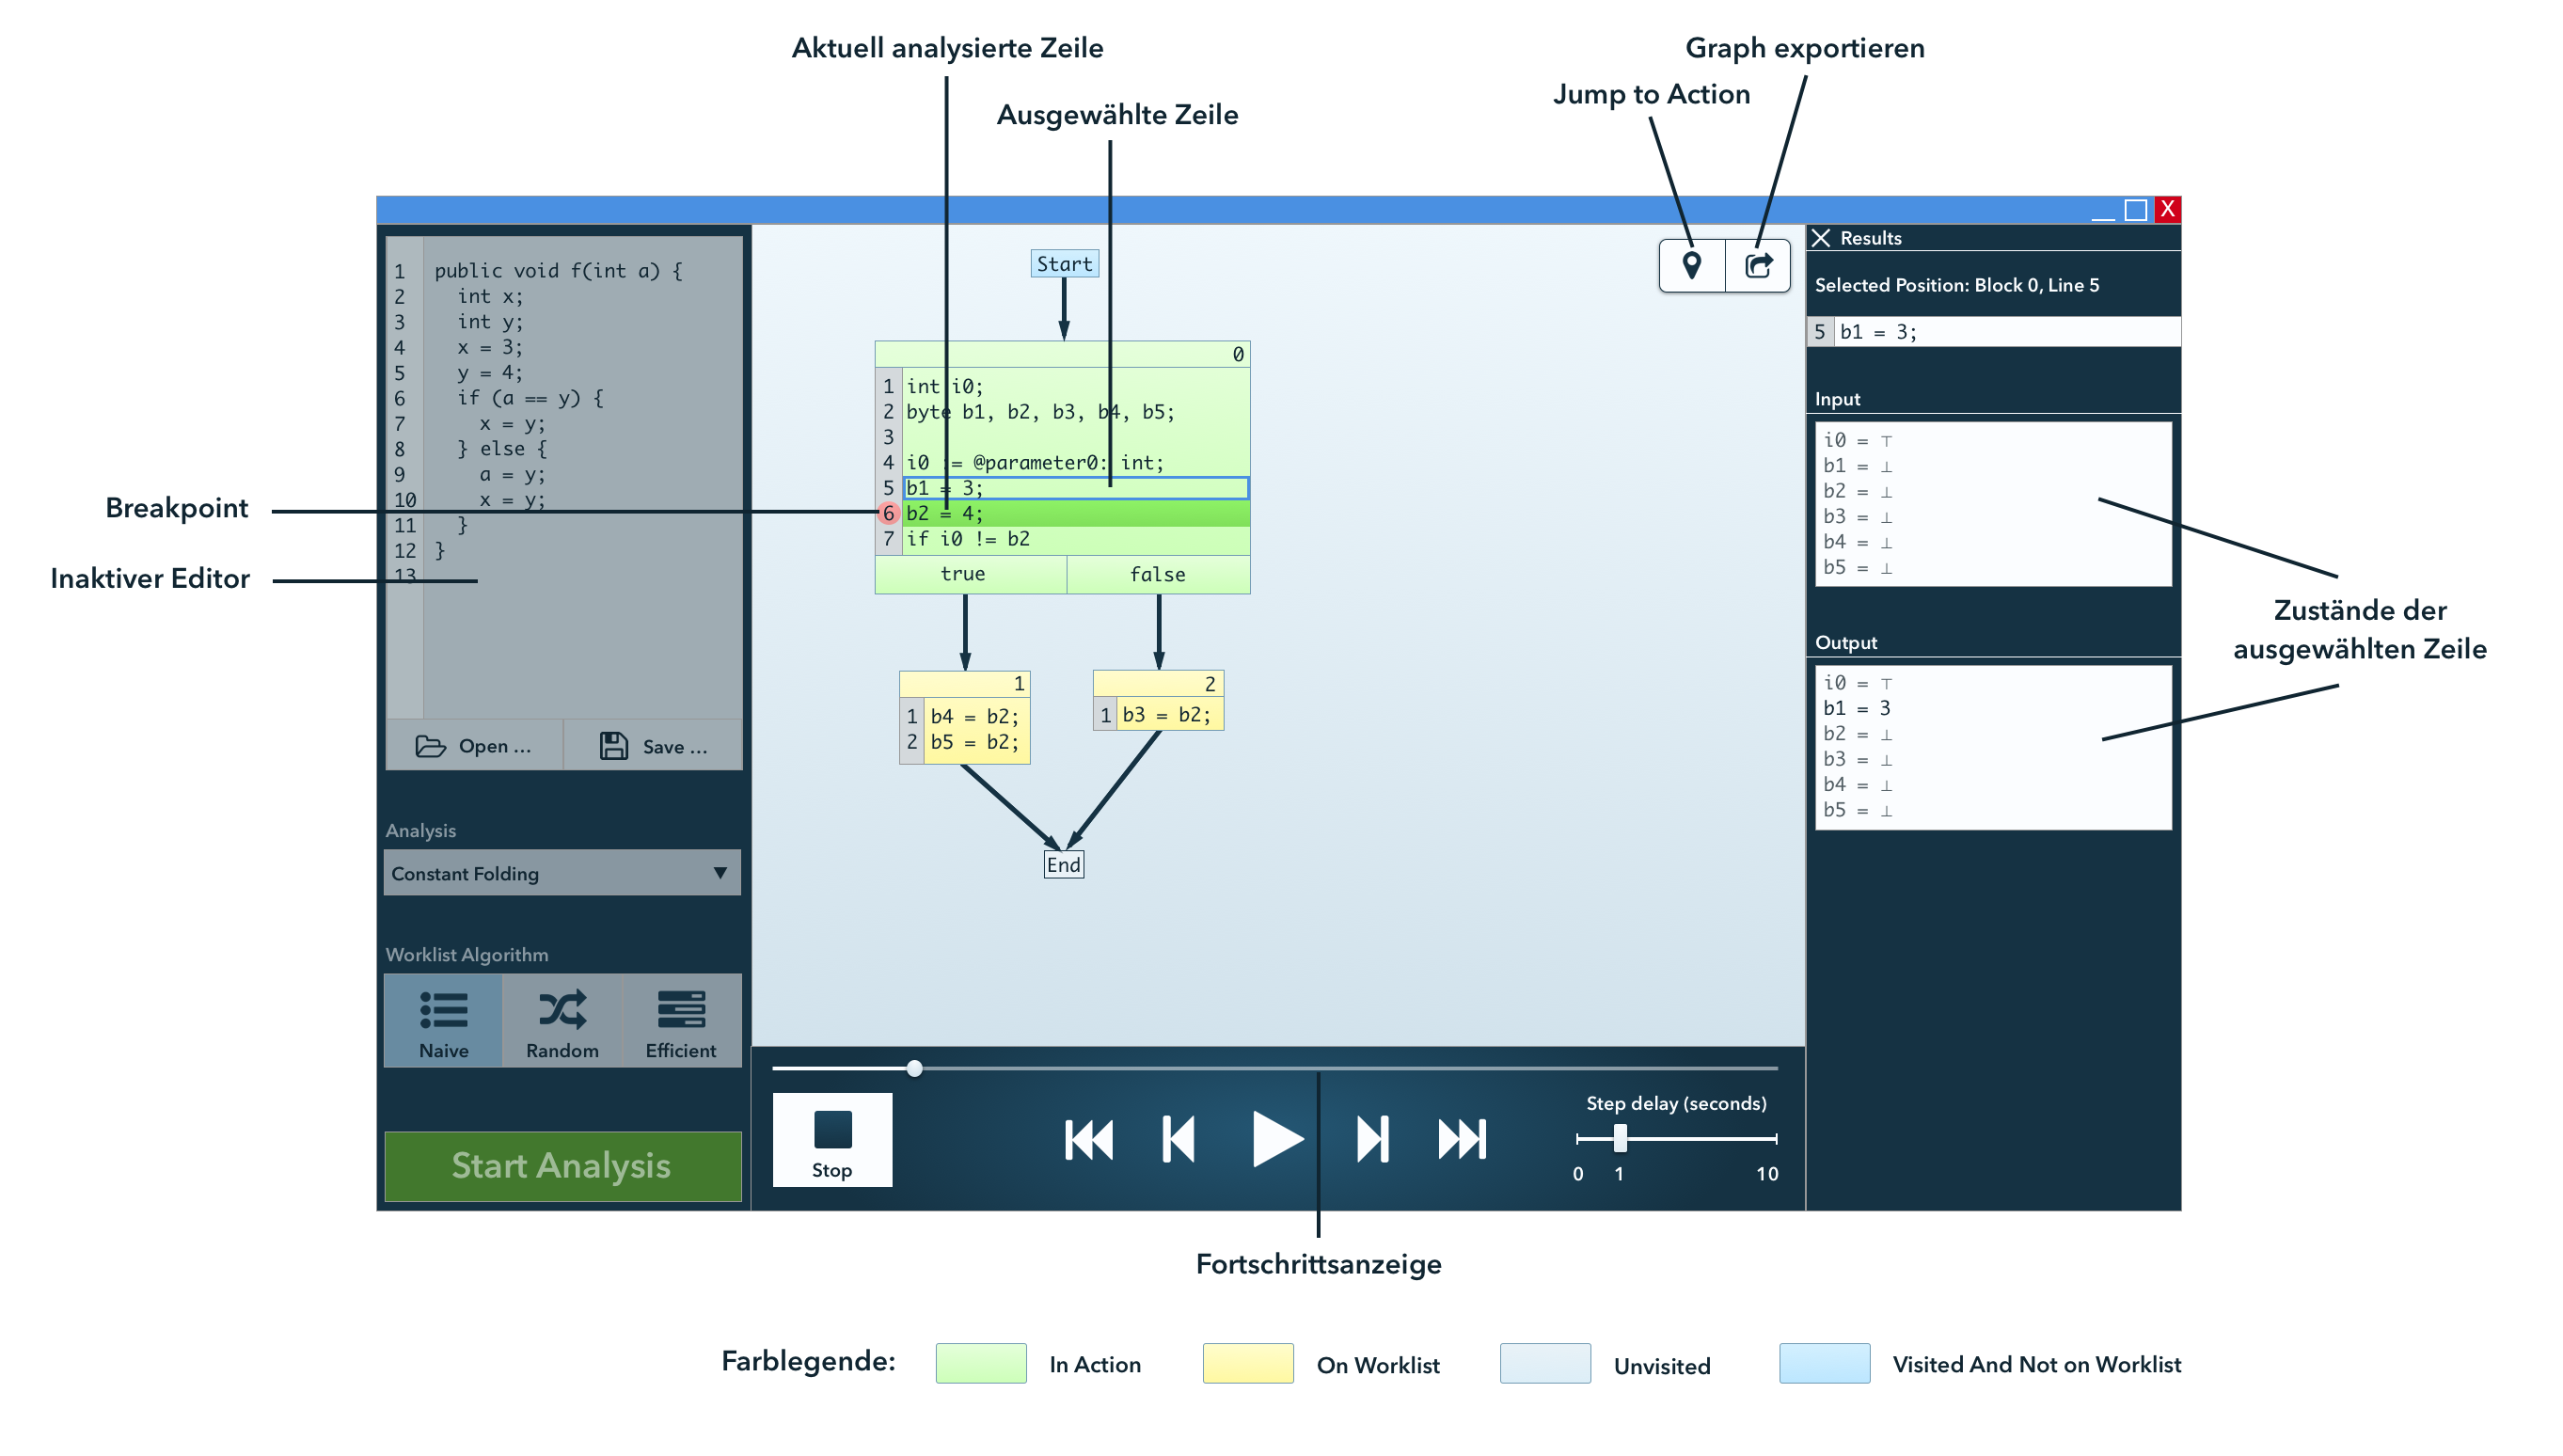
\includegraphics[angle=90, width=0.93\textwidth]{annotated-kann}
\end{figure}

\begin{figure}[H]
\caption{Graph-Export-Dialog}
\centering
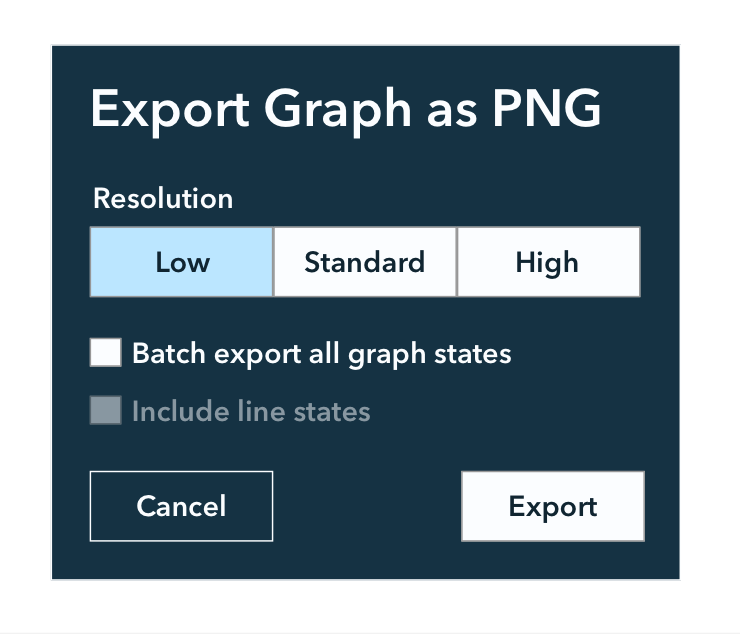
\includegraphics[width=0.6\textwidth]{export}
\end{figure}

\begin{figure}[H]
\caption{Dialog zur Auswahl der analysierten Methode}
\centering
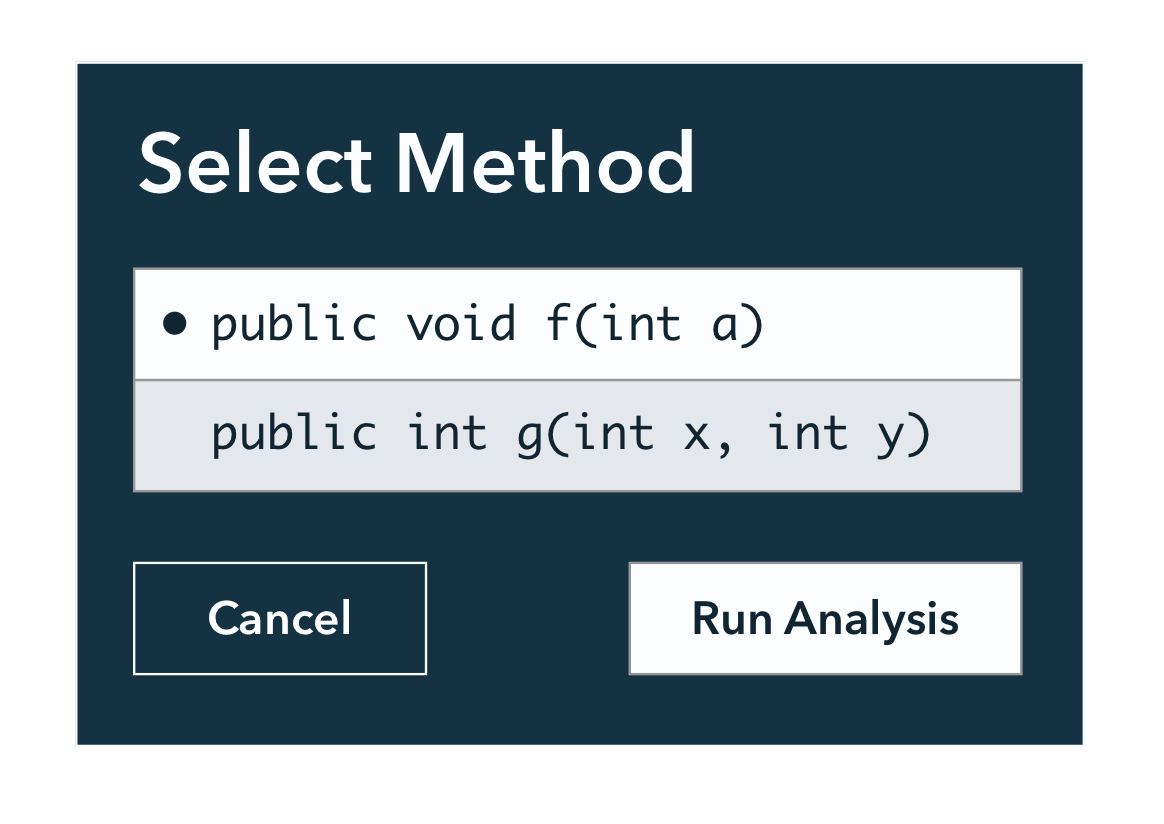
\includegraphics[width=0.6\textwidth]{select-method}
\end{figure}